\documentclass[10pt,a4paper]{scrartcl}
\usepackage[ngerman]{babel}
\usepackage[utf8]{inputenc}
\usepackage[T1]{fontenc}
\usepackage{fancyhdr}
\usepackage{hyperref}
\usepackage{listings}
\usepackage{graphicx}
\usepackage[a4paper,inner=3.5cm,outer=3cm,top=4cm,bottom=3cm,pdftex]{geometry}

\setkomafont{sectioning}{\normalfont\bfseries}

\pagestyle{fancy}
\fancyhf{}
\renewcommand{\headrulewidth}{0.4pt}

\title{XML-Projekt SoSe 2012}
\subtitle{GPSies.org, DBPedia.org, Twitter.com, XML/XSD/XSLT\vspace*{.7cm}}
\author{Gruppe 11\\\hfill\\Eike Cochu, Samer El-Safadi, Hannes Geist,\\Cenk Gündogan, Michael Pluhatsch}
\date{\today}
\fancyfoot[C]{\thepage}
\fancyhead[L]{XML SoSe2012}
\fancyhead[R]{Cochu, El-Safadim, Geist, Gündogan, Pluhatsch, \today}

\setlength\parskip{\medskipamount}
\setlength\parindent{0pt}

\RequirePackage[usenames,dvipsnames]{color}
\RequirePackage{listings}
\lstset{
  language=Java,
  basicstyle=\ttfamily\small,
  numbers=left,
  numberstyle=\tiny,
  numbersep=5pt,
  tabsize=2,
  showstringspaces=false,
  extendedchars=true,
  breaklines=true,
  showtabs=false,
  showspaces=false,
  keywordstyle=\color{orange},
  commentstyle=\color{ForestGreen},
  stringstyle=\color{blue},
  escapechar=@,
  morekeywords={bool,iffalse}
}

\begin{document}
\maketitle
\thispagestyle{empty}
\vspace*{2cm}
\tableofcontents
\newpage
\renewcommand{\baselinestretch}{1.5}
\selectfont

\section{Aufgabenstellung und Organisation}
Gruppenleiter: Hannes Geist

\subsection{Aufgabenstellung}
Durch den XML-Endpoints von gpsies.com 110.000 Wanderstrecken laden, per XSLT-Schema in ein eigens entwickeltes XSD-Schema transformieren und in einer geeigneten XML-Datenbank speichern. Zu diesen Strecken soll per SPARQL der Endpoint von dbpedia.org abgefragt und alle auf (oder an) der Strecke liegenden Sehenswürdigkeiten abgefragt werden können. Ein HTML-Formular (oder ähnliches) entwickeln, mit dem die XML-Datenbank abgefragt werden kann. Das Ergebnis der Abfrage soll wiederum per XSLT in HTML transformiert und zusammen mit den vorhandenen Sehenswürdigkeiten und den zu diesen Sehenswürdigkeiten vorhandenen Tweets von Twitter.com angezeigt werden.

\subsection{Organisatorisches}
Zur Gruppenkoordinierung hat sich unsere Gruppe jede Woche Sonntags beim Gruppenleiter Hannes Geist getroffen und das weitere Vorgehen besprochen und gemeinsam an den einzelnen Softwarekomponenten gearbeitet. Diese Dokumentation ist gemeinsam entstanden, wobei jeder seinen Aufgabenteil beschrieben und etwaige Probleme, die im Verlauf der Bearbeitung auftraten, aufgezählt und ausgeführt hat.

Die endgültigen Ergebnisse sind momentan noch unter \href{http://cochu.dyndns.org/xml} erreichbar, die Präsentationen der Meilensteine sind als PDF beigelegt.

\subsection{Aufgabenverteilung und -bewältigung}
\begin{itemize}
\item Eike Cochu: Erstellung des XSD-Schemas, Bereitstellung eines Servers, Dokumentation
\item Samer El-Safadi: SPARQL-Abfrage der Sehenswürdigkeiten von dbpedia.org
\item Hannes Geist: XSLT-Transformierungen und Füllen der XML-Datenbank
\item Cenk Gündogan: Abfrage der Strecken von gpsies.org 
\item Michael Pluhatsch: HTML-Formular mit PHP, Abfrage der XML-Datenbank
\end{itemize}

% ------------------------------------------------------------------------------
% Teil mit den individuellen Aufgabenbeschreibungen, jeder hat seine eigene 
% .tex-Datei! Text dazu bitte nicht hier reinschreiben
% Inhalt eures Textes: Aufgaben, die ihr erledigt habt, wie und mit was ihr sie
% erledigt habt, was ihr für Probleme hattet usw.
\subsubsection{Eike Cochu}
Aufgabenbereich: Erstellung eines XSD-Schemas für die XML-Datenbank, Bereitstellung des Datenbank- und Applikationsservers sowie Installation der Datenbank, Einfügen der Inhalte in die Datenbank und Installation der Webseite, kleine kosmetische Änderungen an der Webseite und Formatierung, Erstellen der Dokumentation.

\paragraph{XSD-Schema}
Nachdem wir uns mit einem kurzen Testlauf einige Anschauungsdaten von gpsies.org beschafft hatten, konnten wir basierend darauf grob die Anforderungen an das XSD-Schema entwerfen. Die Idee des Schemas sollte es sein, mehr mit Attributen zu arbeiten und so die Anzahl an Elementen zu verringern, damit die Speichergröße der resultierenden Dateien minimal gehalten wird. Dazu haben wir uns entschlossen, einige weniger wichtige Datenteile der crawl-Daten garnicht erst mit in die Datenbank zu speichern, im Schema waren diese dann auch nicht vorgesehen. Die meisten Elemente sind mittels minOccurs=0 ebenfalls optional gehalten, Attribute sind per default optional.

Zur Veranschauung ein kleiner Ausschnitt aus dem Schema:

\begin{lstlisting}[language=XML]
<!-- Eine Adresse. Optional: alles -->
<xsd:complexType name="address">
  <xsd:attribute name="street" type="xsd:string"/>
  <xsd:attribute name="streetnumber" type="xsd:string"/>
  <xsd:attribute name="zipcode" type="xsd:string"/>
  <xsd:attribute name="city" type="xsd:string"/>
  <xsd:attribute name="country" type="xsd:string"/>
</xsd:complexType>
\end{lstlisting}

Hier ist zu sehen, dass in unserem Schema hauptsächlich Attribute verwendet werden, um die Anzahl an Elementen zu verringern. Auch sind Attribute standardmäßig optional, was bei Elementen erst hätte eingerichtet werden müssen.

Beim Schema sind wir auf keine Probleme gestoßen. Das XSD erlaubt es auf einfache Art und Weise ein sehr dynamisches Schema zu erstellen, dass wir im Prozess der Entwicklung aufgrund von neuen Erkenntnissen immer wieder verädert haben, bis es allen Anforderungen entsprach. Die Validierung des Schemas wurde mit einem gewöhnlichen XSD-Schemavalidierer durchgeführt, der unser Schema mit dem eigentlichen XSD-Schema validieren konnte.

\paragraph{Datenbank}
Wir haben uns für BaseX als Datenbank entschieden, da dieses auf Java basiert und somit systemunabhängig installierbar und auch leicht zu handhaben ist. Die Datenbank wurde auf einem dedizierten Ubuntu 12.04 Server installiert, als Webserver wurde Apache + PHP 5 gewählt.

Probleme mit der Datenbank: Da das entgültige Datenbankfile eine Größe von ~1.2 GB hatte und der Heapspeicher der JVM default sehr klein ist, trat beim Erstellen der Datenbank immer ein Out Of Memory Fehler auf, den ich erst mit dem manuellen hochsetzen des Heapspeichers beheben konnte ({\tt java -cp basex.jar org.basex.BaseXServer -Xmx1G}). Bei genauerer Untersuchung habe ich herausgefunden, dass dieser Speicherfehler speziell durch die Volltextindizierung ausgelöst wird, die auch gezieht ausgeschaltet werden kann. 

\subsubsection{Samer El-Safadi}
Bei der Aufgabe die XML-Datenbank um relevante "`Points of interest"'-Daten
zu erweitern, sind wir uns sehr schnell einig gewesen, uns auf Deutschland
zu konzentrieren und sämtliche andere Länder außer Acht zu lassen.\\

Um an jene Punkte zu kommen, mussten wir uns erst einmal über die
Abfragesprache SPARQL informieren. Dies haben wir größtenteils über das
Buch "`Learning SPARQL"' von Bob DuCharme getan, in dem sowohl allgemeine
Informationen über die Materie (sprich das "`Semantic Web"', RDF, Linked
Data etc.), als auch spezielle Situationen dargestellt sind, die über
SPAQL-Abfragen anschaulich bearbeitet werden. Praktischerweise beziehen
sich einige der Beispiele direkt auf DBpedia, wodurch wir das Geschriebene
auch gleich testen konnten.\\

Nachdem wir damit nun eigene Abfragekonstrukte erstellen konnten, die wir
über den Online-Zugriff ausprobiert haben, ging es nun darum den
SPARQL-Endpoint nun auch über Java ansprechen zu können. Schnell fiel die
Wahl auf das Jena Framework von Apache, welches uns einen sehr
komfortablen Weg ermöglichte über ARQ auf den entsprechenden Endpunkt
zuzugreifen: Wir konnten also durch die QueryFactory entsprechende
Anfragen erstellen und diese über QueryExecutionFactory.sparqlService an
einen definierten Service (in diesem Fall DBpedia) senden.\\

Das Programm machte uns durch Warnungen darauf aufmerksam, dass kein
Logger eingerichtet worden ist. Wir behoben dies gleich und integrierten
log4j (ebenfalls Apache), um die Ergebnisse der Anfrage in ein Logfile zu
schreiben, statt es nur (testweise) in die Standardausgabe zu packen.
Als dies erledigt war, konnten wir über die Ergebnisse (ResultSet)
iterieren (.hasNext() bzw. .next()) und diese dann über den Logger direkt
in eine Datei schreiben.

Da das Ergebnis allerdings ein XML-Dokument sein sollte, um es über XSLT
entsprechend einfach umzuwandeln, mussten wir erstmal eine Art Parser
schreiben, der über die Iteration der Ergebnisse ein wohl geformtes
XML-Dokument erstellt.

Dies funktionierte zwar, stellte sich allerdings als sehr aufwendig
heraus, so dass wir uns nach einer neuen Lösung umgesehen haben: Jenas
ResultSetFormatter.outputAsXML war die perfekte Lösung unserer Probleme.\\

Wir mussten entsprechend umdisponieren, haben den log4j-Logger wieder
entfernt und entsprechend mit dem Fileoutputstream gearbeitet, den wir
komfortabel über den ResultSetFormatter von Jena dazu bringen konnten uns
die Ergebnisse in eine sehr übersichtliche XML-Datei zu parsen.\\

Nun stand das Programm und es ging darum unsere Abfragekonstrukte durch
sinnvolle Abfragen zu ersetzen. Dafür mussten wir viel Zeit investieren,
um uns erst einmal einen Überblick zu verschaffen, wie die Datensätze in
der DBpedia angeordnet waren. Wir merkten schnell, dass die englische
DBpedia weitaus weniger relevante Daten über Deutschland enthielt, als die
deutsche - die allerdings wiederum weitaus weniger GEO-Datensätze über die
entsprechenden Objekte enthielt (vergleiche http://de.dbpedia.org/page/Brandenburger\_Tor\\
mit http://dbpedia.org/page/Brandenburg\_Gate).\\

Außerdem mussten wir feststellen, dass viele Objekte oftmals falsch bzw.
scheinbar keiner Regel folgend in entsprechende Typen eingeordnet wurden
und alles doch recht chaotisch war, sodass wir nicht einfach eine große
Anfrage starten konnten und die Ergebnisse anschließend anhand ihrer Typen
zuordnen konnten. Wir verbrachten viel Zeit damit die yago-Sprachklasse
bzw. die Kategorien von DBpedia zu studieren, um entsprechend gezielte
Anfragen zu stellen. Mindestvoraussetzung eines Objektes war für uns die
Bezeichnung, Geo-Daten in Form von long und lat sowie ein Link zum
entsprechenden Wikipedia-Artikel, damit der Nutzer sich weitere
Informationen einholen konnte.\\

Durch dieses Vorgehen waren wir in der Lage Anfragen zu entwickeln, die
relativ schnell abgearbeitet wurden und wir wussten genau, um welche
Untermenge es sich bei den Ergebnissen handelte, sodass wir dies
entsprechend in der Datenbank vermerken konnten. Dadurch konnten wir die
Website entsprechend so einrichten, dass der Nutzer es sich einzeln
aussuchen konnte, ob dieser Parks, Seen etc. angezeigt bekommen wollte
oder nicht.

\subsubsection{Hannes Geist}

\subsubsection{Cenk Gündogan}
Aufgabenbereich: Entwerfen und Implementieren eines Crawlers, 
der mind. 100.000 Tracks vom gpsies.org Server herunterlädt und lokal in einer gültigen 
XML-Datei abspeichert.\\

Bei der Entwicklung des Crawlers wurden die Eigenschaften "`Stabilität"' und "`Schnelligkeit"' sehr
hoch priorisiert. "`Stabilität"' bedeutet, dass der Crawler bei Verbindungsabbrüchen weiter arbeiten
kann und als Resultat immer noch eine korrekte XML-Datei mit gültigem Inhalt produziert wird.
"`Schnelligkeit"' des Crawlers wird durch Parallelisierung des Verbindungsaufbaus zum Server gewährleistet.
Eine weitere nennenswerte Eigenschaft ist die Tatsache, dass das Resultat des Crawlers in komprimierter
Form (mit gzip) erstellt wird. Das Ergebnis ist dann sehr einfach und unproblematisch auf verschiedene
Rechner übertragbar.\\

Die Anfragen an den Server geschehen via Http POST und sehen folgendermaßen aus:

\begin{tabular}{|c|p{10cm}|}
  \hline
    key		&	der API-Key wurde von gpsies.org bereitgestellt. Ohne diesen ist eine Anfrage
			an den Server nicht möglich\\\hline
    country	&	wir beschränken uns nur auf Tracks aus Deutschland\\\hline
    filetype	&	Als Dateityp der GPS-Daten erwarten wir KML\\\hline
    limit	&	es sollen \textbf{limit} viele Track-Ids übertragen werden\\\hline
    resultpage	&	pro Query können immer nur 100 Tracks übermittelt werden, mit
			inkrementierender \textbf{resultpage} kann man die nächsten 
			100 Tracks abfragen\\\hline
\end{tabular}

\begin{enumerate}
  \item URL1: \textit{http://www.gpsies.org/api.do?\textbf{key}=<key>\&\textbf{country}=DE\&
	\textbf{limit}=100\&\textbf{resultpage}=i}\\
	Es werden die \textbf{i.}en 100 Tracks geladen
  \item URL2: \textit{http://www.gpsies.org/api.do?\textbf{key}=<key>\&\textbf{limit}=100
    \&\textbf{filetype}=kml\&\textbf{fileId}=f1\&\textbf{fileId}=f2\ldots}\\
	Die 100 TrackIds, die mit URL1 erfragt wurden, werden nun alle an die 2. URL angefügt.
	Mit URL2 erhalten wir detaillierte Informationen zu jedem Track
\end{enumerate}

Zur Realisierung des Crawlers wurde ein Maven-Projekt erstellt und zur leichten Handhabung
der REST-Abfragen der HttpClient von org.apache.httpcomponents benutzt. Die Programmiersprache ist Java.

Der Crawler besteht aus zwei Hauptkomponenten, dem Master und die Worker.
Zuerst wird vom Master ein komprimierter Output-Stream(gzip), verknüpft mit einer lokalen Datei, geöffnet.
Der Master stellt nun in einer Schleife, die von \textbf{i=0} bis \textbf{i=\textit{iterations}} geht,
die Anfrage (URL1) an den Server, um die \textbf{i.}en 100 TrackIds zu erhalten. Aus der Response des
Servers werden mittels regular expression die einzelnen TrackIds heraus gefiltert. Mit den erhaltenen
TrackIds kann nun die zweite Abfrage an den Server gestellt werden (URL2), um detaillierte Informationen
zu jedem Track zu erhalten. Diese zweite Response wird nun wieder mittels regular expression 
nach Tracks untersucht. Bei jedem Fund eines Tracks, wird ein Worker erzeugt und 
diesem der gefundene Track übergeben.
Der Master wiederholt diesen Prozess bis keine weiteren Tracks in der Response gefunden werden und
wartet auf die Terminierung aller Worker. Wenn alle Worker terminiert sind, entsteht ein 
gültiger XML-Abschnitt, der in den komprimierten Output-Stream geschrieben und geflusht werden kann.
Nun beginnt die nächste Iteration des Masters und dieser Prozess führt sich fort, bis 
\textbf{i=iterations} erreicht ist.

Wird ein Worker erstellt und ihm ein Track übergeben, wird der Download-Link der KML-Datei dieses Tracks
via regular expressions heraus gefiltert. Die KML-Datei wird mit einem InputStreamReader geöffnet und
die enthaltenen Koordinaten ausgelesen. Wir entschieden uns hierbei für eine "`nimm jede 10."'-Politik,
da es überaus viele, sehr dicht beieinander liegende, Koordinaten zur Verfügung gab.
Zum Beenden des Workers wird der Track samt ausgelesener Koordinaten an den Master übergeben.

Das Resultat ist eine komprimierte XML-Datei mit 100.000 Tracks + Koordinaten. Die Größe der Datei
liegt bei ungefähr $\sim$200MB. Entpackt liegt die Größe bei $\sim$1.1GB.
Die ideale Crawl-Dauer liegt bei $\sim$3.5h-4h\\

Aufruf des Crawlers: {\tt java -jar ./crawler "`api-key"' "`/path/to/file.xml.gz"' "`number of iterations"'}\\
Die Dateiendung muss "`gz"' sein, da eine komprimierte Datei erzeugt wird. Eine Iteration beinhaltet 
im besten Fall 100 Tracks, so erhält man bei 1000 Iterationen 100.000 Tracks.\\

Probleme: Das schwerwiegenste Problem war die Tatsache, dass der Crawler aufgrund von langen Ausfallzeiten
seitens des Servers nicht genügend Tracks produzieren konnte und durch viele Timeouts um mehrere Stunden
verlangsamt wurde.


\subsubsection{Michael Pluhatsch}

% ------------------------------------------------------------------------------

\section{Installation und Systemvoraussetzungen}

Zur Installation wird ein Webserver + PHP und BaseX als XML-Datenbankserver benötigt. Die web-Dateien gehören in ein Unterverzeichnis in den Documentroot des Webservers. Die Datenbank wird mittels
\begin{verbatim}
$ java -cp basex.jar org.basex.BaseXServer -Xmx1G
$ java -cp basex.jar org.basex.BaseXClient
$ > create db db-crawl <input-file.xml>
\end{verbatim}

erstellt und der Datenbankserver gestartet. Erst dann kann das PHP-Script der Hauptseite auf die Datenbank zugreifen.

Als Systemvoraussetzungen gelten eine Mindestmenge von 2GB RAM für das Erstellen und effiziente Durchsuchen der Datenbank.

\section{Systembeschreibung}

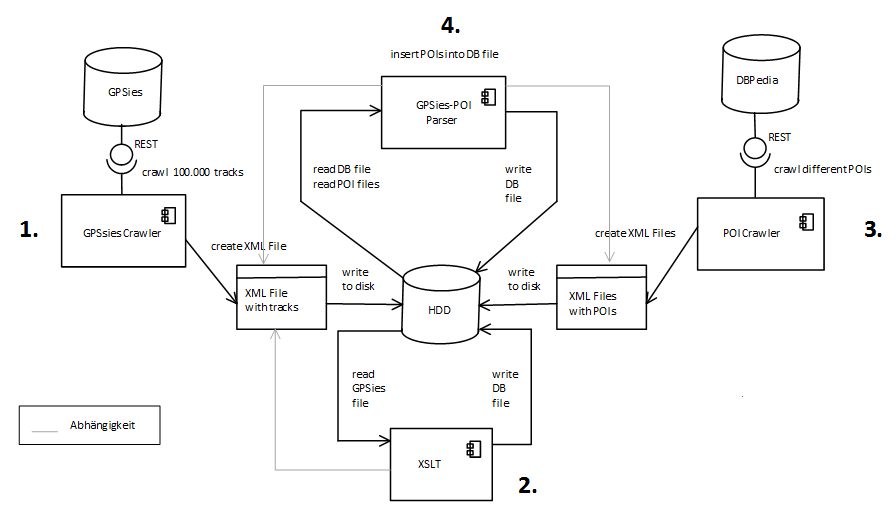
\includegraphics[width=\textwidth]{run_once_schema.png}

Datenbank (1): Der Crawler fragt die Tracks und deren KML-Geopoints per REST-Anfragen bei gpsies.org an und speichert diese zusammen in einer Datei. Ein weiterer Crawler (3) fragt die POI-Daten der dbpedia per SPARQL ab und speichert diese in nach Art des POIs getrennten XML-Dokumenten ab. Dann wird das XML-Dokument mit den Tracks durchlaufen und zu jedem Track die entsprechenden POIs aus den POI-Dokumenten hinzugefügt. Per XSLT-Stylesheet (2) wird diese Datei dann in unser XSD-Schema transformiert. Das so entstandene schemakonforme XML-Dokument wird zur Erstellung der XML-Datenbank benutzt (manuell).

Oberfläche: Per PHP wird eine Anfrage an den Datenbankserver gestellt, das Ergebnis wird wiederum durch PHP interpretiert und als Ergebnis auf der Suchseite dargestellt, die im Track enthaltenen KML-Geopunkte werden über ein Plugin an Google Maps übergeben, wodurch auf der Karte eine visuelle Darstellung des Tracks entsteht.

\section{Benutzung}
Der POInter wird folgendermaßen benutzt:
Mit dem Öffnen der Url (http://cochu.dyndns.org/xml/) gelangt man zur Startseite des POInters.
Diese besteht aus einem Suchfeld und einem Button zum Starten der Suchanfrage.
Zusätzlich ist es möglich vor dem Abschicken der Suchanfrage mehrere Checkboxes auszuwählen,
um sich in der nähe des Tracks befindende POIs in der jeweiligen Kategorie anzuzeigen.
Generell unterscheidet die Suche bei dem Suchwort nicht in der Klein- und Großschreibung!
Nach dem Abschicken der Suchanfrage, sucht der Server das Resultat zusammen und zeigt dem Nutzer alle gefundenen
Tracks tabellarisiert an.
In dieser Tabelle ist der Track Titel und das Erstellungsdatum des Tracks vorhanden.
Klickt man nun auf einen Track, öffnet sich eine Karte mit der ausgewählten Strecke eingezeichnet.
Mit dem Klick auf den Startpunkt, erhält man sämtliche Informationen zum Track, außerdem werden alle
gefundenen POIs der gewünschten Kategorie, die zum Track zugeordnet sind, auf der Karte angezeigt.


\end{document}
